\section{رویکرد دیگر برای تجزیه SVD برای ابعاد بالاتر}
\begin{frame}[standout]
T-SVD
\end{frame}
\begin{frame}
{تعاریف مقدماتی}
\metroset{block=fill}
 \begin{alertblock}{ماتریس پیچشی}
	 تانسور سه بعدی
	$\mathcal{A}\in\mathbb{R}^{l\times m\times n}$
	با $l\times m$ اسلایس پیشی مفروض است. در این صورت
	\begin{tabular}{p{0.7cm}cc}
	 	&
	$
	circ(\mathcal{A})=\begin{pmatrix}
	A^{(1)}&A^{(n)}&A^{(n-1)}&\cdots &A^{(2)}\\
	A^{(2)}&A^{(1)}&A^{(n)}&A^{(n-1)}&\cdots \\
	\vdots &\ddots&\ddots&\ddots&\vdots\\	
	A^{(n)}&A^{(n-1)}&\cdots &A^{(2)}&A^{(1)}\\
	\end{pmatrix}
	$
	&
\end{tabular}
که ماتریس پیچشی بلوکی از سایز 
$ln\times mn$
است.
\end{alertblock}
\end{frame}
\begin{frame}{T-Prudact}
\metroset{block=fill}
\begin{exampleblock}{عملگرهای $fold$ و $MatVec$}
	عملگر $MatVec$ تانسور سه بعدی به ابعاد 
	$l\times m\times n$
	را به ماتریس بلوکی با ابعاد 
	$ln \times m$
	برمی‌گرداند و عملگر $fold$ معکوس این عملگر را انجام می‌دهد.
	
	\begin{tabular}{p{0.9cm}ccc}
&$	MatVec(\mathcal{A})=\begin{pmatrix}
A^{(1)}\\A^{(2)}\\\vdots\\ A^{(n)}\\
\end{pmatrix}$&
$fold(MatVec(\mathcal{A}))=\mathcal{A},$&
	\end{tabular}
\end{exampleblock}
\end{frame}
\begin{frame}
\small{
\metroset{block=fill}
\begin{alertblock}{$t$-ضرب}
	فرض کنید 
	$\mathcal{A}\in \mathbb{R}^{l\times p\times n}$
	و
	$\mathcal{B}\in \mathbb{R}^{p\times m\times n}$.
	در این صورت $t$-ضرب با ابعاد
	$l\times m\times n$
	را به صورت 
	$\mathcal{A} \star \mathcal{B}$
	نشان داده و به صورت زیر تعریف می‌شود.
	
	\begin{tabular}{p{1.3cm}cc}
		&$\mathcal{A} \star \mathcal{B}=fold\left(circ(\mathcal{A}) MatVec(\mathcal{B})\right).$
	\end{tabular}

\pause
این ضرب در حالت کلی خاصیت جابجایی ندارد.
\end{alertblock}

\pause
\metroset{block=fill}
\begin{alertblock}{تبدیل فوریه گسسته ($DFT$)}
	ماتریس مربعی $F$ با ابعاد $N$ در $N$ را به صورت
	$F=\left(\frac{w^{jk}}{\sqrt{N}}\right)_{j,k=0,\cdots,N-1}$
	که در آن
	$\omega=e^{-2\pi i/N}$ 
	است.
	 به صورت ماتریس داریم:	
	\begin{center}
		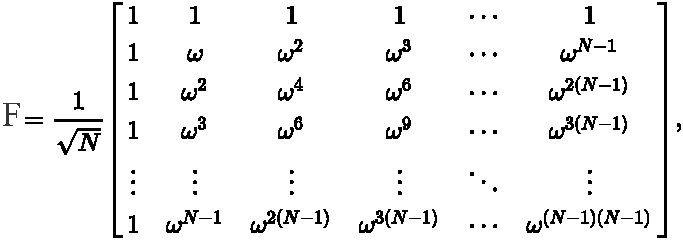
\includegraphics[width=0.5\textwidth]{img/ok/DFTW.pdf}
	\end{center}
\end{alertblock}
}
\end{frame}
\begin{frame}{T-SVD}
هرگاه $F$ ماتریس نرمال شده تبدیل فوریه باشد، برای 
$\mathcal{A}\in \mathbb{R}^{l\times m\times n}$،
$n$
ماتریس با درآیه‌های مختلط
$\hat{A}^{(i)}$
با ابعاد 
$l\times m$
وجود دارد به طوریکه:
\[(F\otimes I)circ(\mathcal{A})(F^*\otimes I)=
\begin{pmatrix}
\hat{A}^{(1)} & 0 &\cdots & 0\\
0&\hat{A}^{(2)}&\cdots & 0\\
\vdots&\ddots&\ddots&\vdots\\
0&0&\cdots&\hat{A}^{(n)}
\end{pmatrix}=\hat{\mathcal{A}},
 \]
 اما نیاز نیست که به صورت صریح
 $\hat{\mathcal{A}}$
 از 
 $circ(\mathcal{A})$
 تولید شود. با  تبدیل فوریه  از مد سوم تانسور $\mathcal{A}$
 تانسور 
  $\hat{\mathcal{A}}$،
  تولید می‌شود.
  
  \pause
  توجه: برای تانسور $\mathcal{A}$ و $\mathcal{B}$
  داریم:
  \[\mathcal{A}\star \mathcal{B}=\mathcal{C} \Longleftrightarrow \hat{\mathcal{A}}\hat{\mathcal{B}}=\hat{\mathcal{C}} \]
\end{frame}
\begin{frame}{T-QR and T-SVD}
\metroset{block=fill}
\begin{alertblock}{تجزیه $T-QR$}
	با استفاده از تعریف فوق می‌توان تانسور $\mathcal{A}$ را بصورت
	$\mathcal{A}=\mathcal{Q}\star \mathcal{R}$
	نوشت که در آن
	$\mathcal{Q}$
	معکوس تبدیل فوریه 
	$\hat{\mathcal{Q}}$
	مد 3 است.
\end{alertblock}

\pause
\metroset{block=fill}
\begin{exampleblock}{تجزیه $T-SVD$}
با استفاده از تعریف  می‌توان تانسور $\mathcal{A}$ را بصورت
$\mathcal{A}=\mathcal{U}\star\mathcal{S}\star \mathcal{V}^\trans$
نوشت.
\end{exampleblock}
\end{frame}
\begin{frame}{T-SVD}
تجزیه $t-SVD$ که در آن $\mathcal{S}$ 
تانسور قطری است به فرم زیر نشان داده می‌شود.

\pause
	\begin{center}
	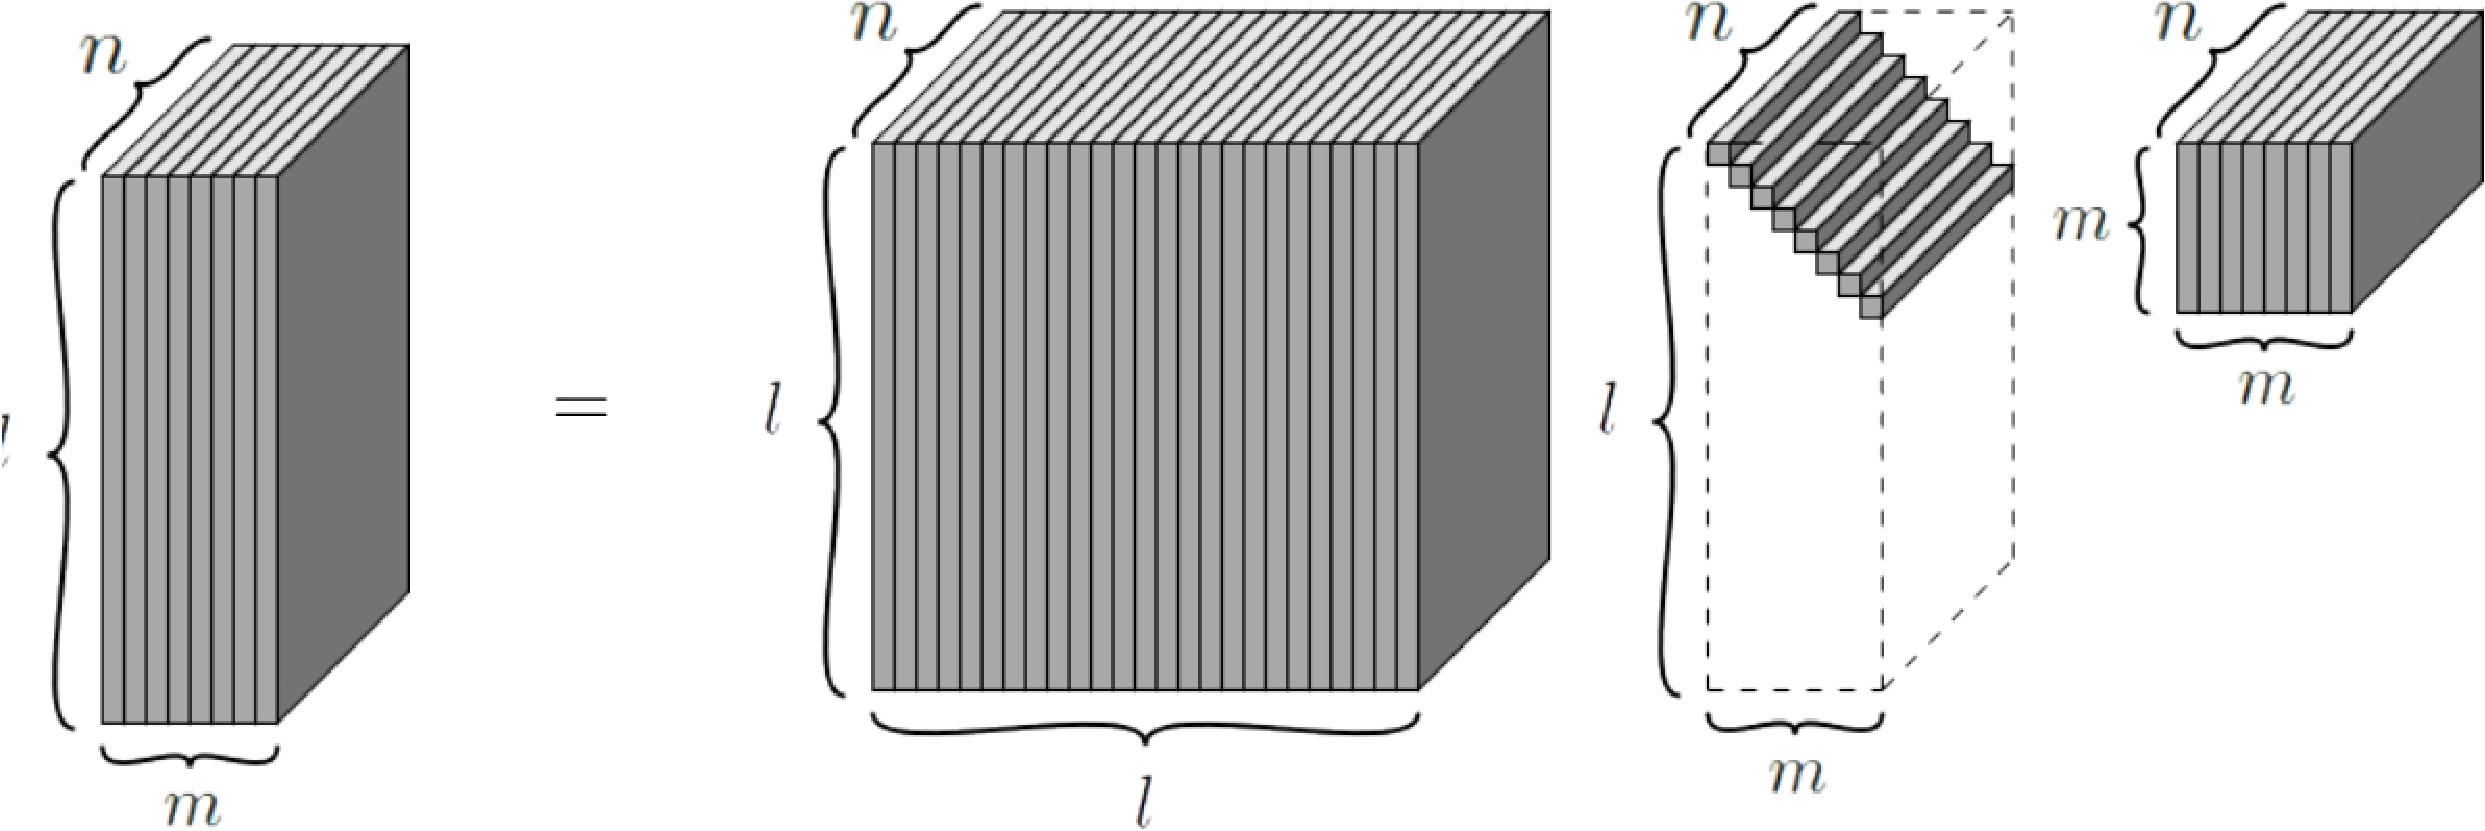
\includegraphics[width=1\textwidth]{img/ok/T-SVD.pdf}
\end{center}
\end{frame}
\begin{frame}
الگوریتم $t-SVD$ برای تانسور سه بعدی به صورت زیر است:
\begin{center}
	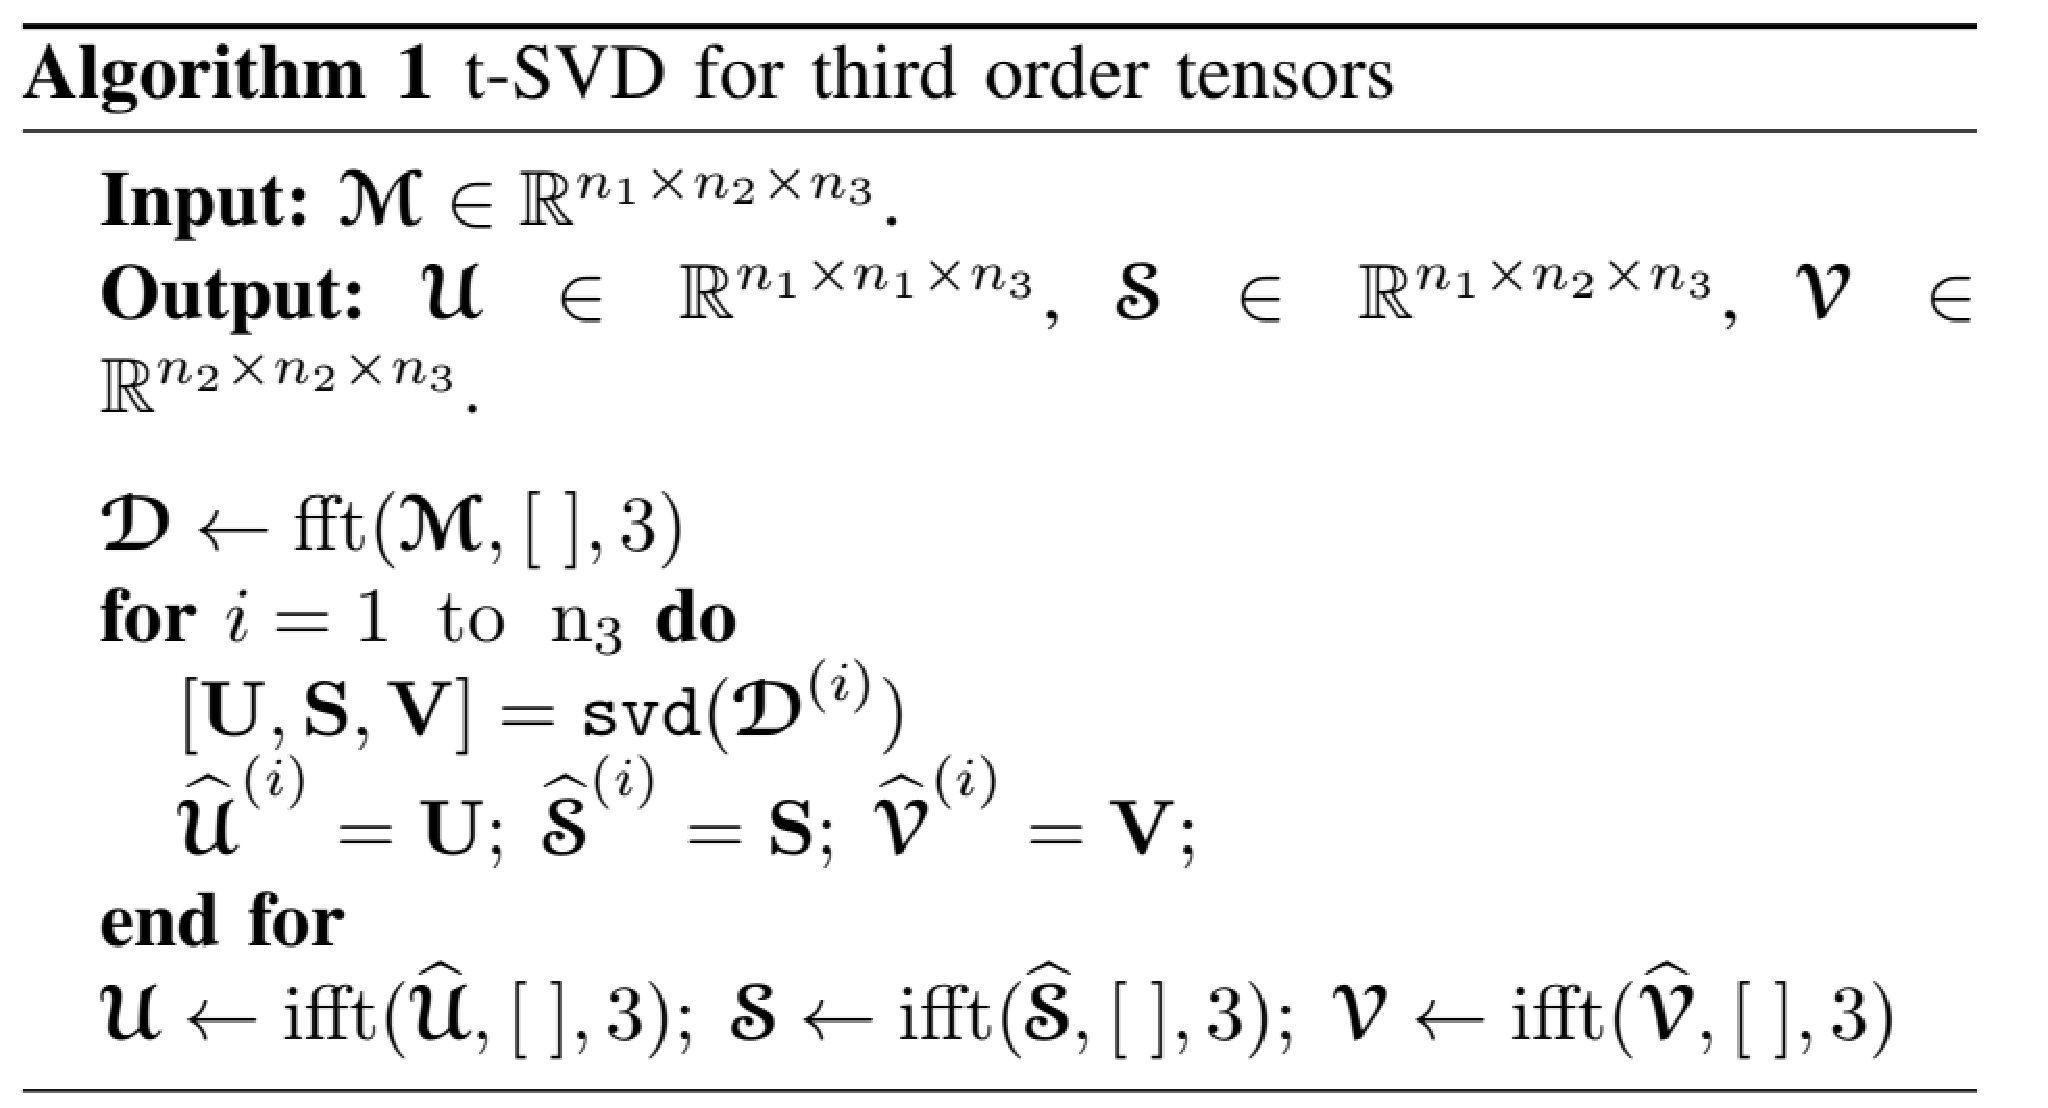
\includegraphics[width=0.8\textwidth]{img/ok/AT-SVD.pdf}
\end{center}
\end{frame}
\begin{frame}

	1 تعریف معین مثبت. 
	\\
	
	\pause
	2 تانسور متعامد\\
	
	\pause
	3 $squeenz$

\pause
\begin{center}
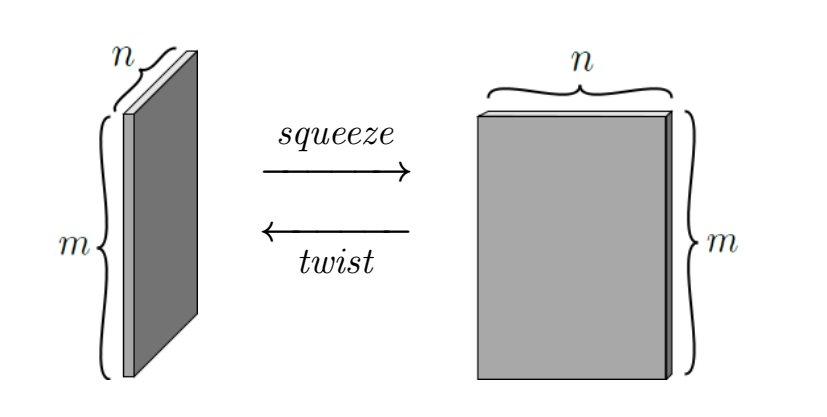
\includegraphics[width=0.8\textwidth]{img/sq.png}
\end{center}
\end{frame}
\begin{frame}{ضرب داخلی}
4 ضرب داخلی برای
$<x,y>:=x^T\star y$

\pause
\begin{center}
	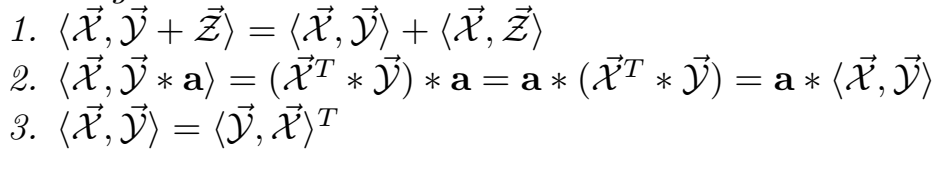
\includegraphics[width=0.8\textwidth]{img/in.png}
\end{center}
\end{frame}
\begin{frame}{کاربرد $TSVD$}
\begin{center}
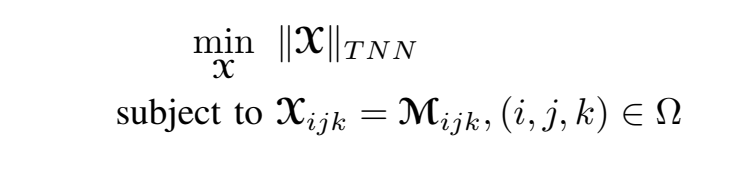
\includegraphics[width=0.8\textwidth]{img/tnn.png}
\end{center}
\end{frame}